\documentclass[11pt,a4paper]{article}
\usepackage[T1]{fontenc}
\usepackage[utf8]{inputenc}
\usepackage{lmodern}
\usepackage[margin=27mm]{geometry}
\usepackage{amsmath,amssymb,amsthm}
\usepackage{booktabs}
\usepackage{microtype}
\usepackage{tikz}
\usepackage[hidelinks]{hyperref}
\usepackage{xurl}
\usepackage{fancyhdr}
\pagestyle{fancy}
\fancyhf{}
\fancyhead[L]{\small Mixed general position in the $9\times9$ grid}
\fancyhead[R]{\small v1.0}
\fancyfoot[C]{\thepage}
\setlength{\headheight}{14pt}
\setlength{\emergencystretch}{2em}

\newtheorem{theorem}{Theorem}[section]
\newtheorem{lemma}[theorem]{Lemma}
\newtheorem{proposition}[theorem]{Proposition}
\theoremstyle{definition}
\newtheorem{definition}[theorem]{Definition}
\theoremstyle{remark}
\newtheorem{remark}[theorem]{Remark}

\newcommand{\Gn}{G_n}
\newcommand{\A}{\mathcal A}
\newcommand{\C}{\mathcal C}
\newcommand{\row}{\operatorname{row}}
\newcommand{\col}{\operatorname{col}}

\hypersetup{
  pdftitle={The Maximum Mixed-General-Position Subset of the 9x9 Integer Grid Has Size 15},
  pdfauthor={Jinchen Li},
  pdfsubject={Computer-assisted proof},
  pdfkeywords={integer grid, general position, concyclic, exhaustive search, proof certificate}
}

\title{The Maximum Mixed-General-Position Subset of the\\$9\times9$ Integer Grid Has Size 15}
\author{Jinchen Li\\\small Independent Researcher, China}
\date{6 September 2026\\[2pt]\small Preprint v1.0}

\begin{document}
\maketitle
\begin{center}
\small DOI: \href{https://doi.org/10.5281/zenodo.22368316}{10.5281/zenodo.22368316}
\end{center}

\begin{abstract}
Let $f(n)$ be the largest size of a subset of the integer grid
$\{0,\ldots,n-1\}^2$ containing neither three collinear points nor four
concyclic points. We give a computer-assisted proof that $f(9)=15$.
The lower bound is an explicit 15-point construction checked by exact integer
arithmetic. The upper bound is certified by a retained exhaustive search tree
with 6,313,888 nodes. A standalone checker rebuilds the forbidden geometric
configurations from the grid coordinates, verifies the capacity bounds and
reconstructs every required branch, so the search producer itself is not part
of the minimal logical argument. A separately implemented pointwise exhaustive
search visits 26,199,928 nodes and reaches the same conclusion. The complete
certificate, checkers, witness and reproduction scripts are publicly archived
in the accompanying GitHub repository. This is a computer-assisted proof, not
a proof-assistant formalization or a claim of completed peer review or priority.
\end{abstract}

\section{Introduction}
For $n\ge2$, let
\[
  \Gn=\{0,\ldots,n-1\}^2.
\]
Call $S\subseteq\Gn$ \emph{admissible} if no three distinct points of $S$
are collinear and no four distinct points of $S$ lie on one genuine Euclidean
circle. Define
\[
  f(n)=\max\{|S|:S\subseteq\Gn\text{ is admissible}\}.
\]
Dong and Xu use the equivalent notation $\operatorname{ex}([n]^2;3,4)$ for
this mixed condition \cite{dongxu2025}.

\begin{theorem}[Computer-assisted]\label{thm:main}
The maximum admissible subset of the $9\times9$ integer grid has size
\[
  \boxed{f(9)=15}.
\]
\end{theorem}

The proof consists of a direct lower-bound witness and a certificate-backed
upper bound. The upper-bound certificate is not accepted merely because a
search program reports ``UNSAT'': a separate checker derives the geometric
constraints and every required child state itself. Section~\ref{sec:soundness}
proves that acceptance of such a complete certificate excludes every
admissible 16-point set.

\section{Related work}
The combined no-three-collinear and no-four-concyclic condition has earlier
antecedents. Thiele's 1995 construction for the no-four-on-circle problem also
enforces the no-three-in-line condition and gives a linear-size mixed
construction \cite{thiele1995}. O'Rourke later posed the combined grid question
explicitly \cite{orourke2018}. Dong and Xu proved the asymptotic lower bound
$\operatorname{ex}([n]^2;3,4)\ge n/3-o(n)$ in dimension two
\cite{dongxu2025}. Recent work on related forbidden configurations and
circle-avoiding grid sets includes \cite{janosik2026,ghosal2026,zhang2026}.

The no-four-on-a-circle problem is sometimes formulated in a way that still
allows collinear triples; such constructions do not automatically solve the
mixed problem studied here. In particular, an audited 18-point $9\times9$
example for the weaker circle-avoidance condition contains collinear triples
and therefore is not a counterexample to Theorem~\ref{thm:main}.

We are not aware of an earlier published determination of this exact mixed
value at $n=9$. This sentence is a literature statement rather than a proof of
priority; the theorem below depends only on the finite certificate and its
verification.

\section{Exact geometry}
For three points $p_i=(x_i,y_i)$, collinearity is equivalent to
\[
  \det\begin{pmatrix}
  x_1&y_1&1\\x_2&y_2&1\\x_3&y_3&1
  \end{pmatrix}=0.
\]
For four points, define the lifted determinant
\begin{equation}\label{eq:circle}
  \det\begin{pmatrix}
  x_1^2+y_1^2&x_1&y_1&1\\
  x_2^2+y_2^2&x_2&y_2&1\\
  x_3^2+y_3^2&x_3&y_3&1\\
  x_4^2+y_4^2&x_4&y_4&1
  \end{pmatrix}.
\end{equation}
A zero value means that the four points are concyclic or collinear. Because
an admissible set already forbids collinear triples, treating every zero
lifted determinant as forbidden is equivalent to the desired circle condition.
All proof-relevant geometry is evaluated with exact signed integers; no
floating-point tolerance is involved.

For $G_9$, independent enumeration gives 2,712 collinear triples and 25,996
genuine concyclic quadruples. There are also 3,156 all-collinear quadruples,
so 29,152 quadruples have zero lifted determinant. These counts are outputs of
the verification code, not premises supplied to the checker.

\section{A 15-point construction}\label{sec:lower}
Consider
\begin{align*}
S_{15}=\{&(0,0),(1,0),(5,1),(7,1),(0,2),\\
&(3,3),(5,3),(7,4),(8,4),(2,5),\\
&(4,5),(6,7),(8,7),(1,8),(2,8)\}.
\end{align*}

\begin{figure}[ht]
\centering
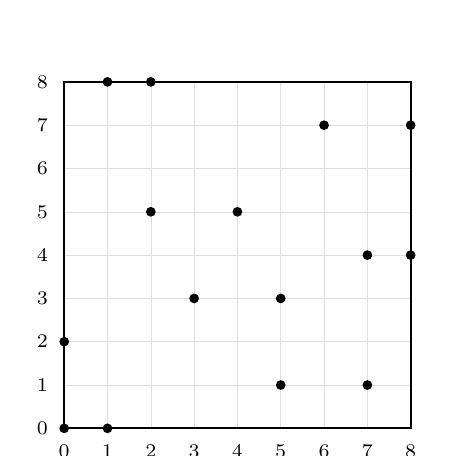
\begin{tikzpicture}[scale=0.55]
  \draw[step=1cm,gray!25,very thin] (0,0) grid (8,8);
  \foreach \x in {0,...,8} \node[below,font=\scriptsize] at (\x,-0.15) {\x};
  \foreach \y in {0,...,8} \node[left,font=\scriptsize] at (-0.15,\y) {\y};
  \foreach \x/\y in {0/0,1/0,5/1,7/1,0/2,3/3,5/3,7/4,8/4,2/5,4/5,6/7,8/7,1/8,2/8}
    \fill (\x,\y) circle (3.2pt);
  \draw[thick] (0,0) rectangle (8,8);
\end{tikzpicture}
\caption{The explicit 15-point witness. The picture is illustrative; exact
integer determinant checks establish admissibility.}
\end{figure}

\begin{proposition}\label{prop:lower}
$S_{15}$ is admissible. Hence $f(9)\ge15$.
\end{proposition}
\begin{proof}[Computer-assisted verification]
The repository contains the machine-readable witness
\path{witnesses/witness15.json}. The independent witness verifier checks the
coordinate range and distinctness and then evaluates all
$\binom{15}{3}=455$ triples and $\binom{15}{4}=1365$ quadruples using exact
integer determinants. None is forbidden.
\end{proof}

\section{Certificate model}\label{sec:model}
Fix a target cardinality $k$. A state $(S,R)$ consists of an admissible
selected set $S$ and a set $R$ of unprocessed horizontal rows, with $S$
disjoint from those rows. A \emph{completion} is an admissible $k$-point set
$T$ with $S\subseteq T$ and every point of $T\setminus S$ lying in a row in
$R$. Let $\C(S,R)$ denote the family of completions.

Define the candidate set
\[
  \A(S,R)=\{p\in\Gn:\row(p)\in R,\;S\cup\{p\}\text{ is admissible}\}.
\]
The checker reconstructs this set from the selected points and the grid
coordinates. Write $A=\A(S,R)$ and $m=k-|S|$. For each row $y$ and column $x$
put
\[
  r_y=|A\cap\row_y|,\qquad c_x=|A\cap\col_x|,
  \qquad u_x=|S\cap\col_x|.
\]
Since an admissible set contains at most two points on any horizontal or
vertical line, define the upper bounds
\begin{equation}\label{eq:bounds}
  B_R=\sum_y\min(2,r_y),\qquad
  B_C=\sum_x\min(2-u_x,c_x).
\end{equation}

\begin{lemma}[Capacity bounds]\label{lem:capacity}
Every completion adds at most $B_R$ points and at most $B_C$ points.
\end{lemma}
\begin{proof}
Every additional point must lie in $A$. A remaining row contributes at most
two admissible points and at most $r_y$ candidates; summing gives $B_R$.
Likewise, a column already containing $u_x$ selected points has residual
capacity at most $2-u_x$, and contains only $c_x$ candidates; summing gives
$B_C$.
\end{proof}

A row-bound leaf is accepted only when $B_R<m$, and a column-bound leaf only
when $B_C<m$. Otherwise the certificate may branch on an unprocessed row
$y\in R$. Let
\begin{equation}\label{eq:lower}
  \ell=\max\{0,m-(B_R-\min(2,r_y))\}.
\end{equation}
The checker itself enumerates every compatible choice
\begin{equation}\label{eq:children}
  Q\subseteq A\cap\row_y,
  \qquad \ell\le |Q|\le\min(2,m),
  \qquad S\cup Q\text{ admissible},
\end{equation}
and recursively requires a certificate for the child
$(S\cup Q,R\setminus\{y\})$. The certificate therefore cannot silently omit
an inconvenient row choice. Zero-child branches are allowed only when the
derived list in \eqref{eq:children} is genuinely empty.

\section{Soundness of the certificate}\label{sec:soundness}
\begin{lemma}[Exhaustive row partition]\label{lem:partition}
For a branch on row $y$, the completion families of the children defined by
\eqref{eq:children} form a disjoint partition of $\C(S,R)$.
\end{lemma}
\begin{proof}
Take a completion $T$ and set $Q=T\cap\row_y$. Each point of $Q$ is in $A$,
$|Q|\le2$, and $S\cup Q$ is admissible. Outside row $y$, the row capacity is
at most $B_R-\min(2,r_y)$, so reaching size $k$ requires
\[
  |Q|\ge m-(B_R-\min(2,r_y)),
\]
hence $|Q|\ge\ell$. Thus this exact $Q$ occurs among the generated children.
Conversely, any completion of a child is a completion of the parent. Distinct
choices $Q$ have distinct intersections with the processed row $y$, so the
families are disjoint.
\end{proof}

\begin{theorem}[Certificate soundness]\label{thm:sound}
If the complete certificate for parameters $(n,k)$ is accepted at the root
$(\varnothing,\{0,\ldots,n-1\})$, then no admissible $k$-point subset of
$G_n$ exists.
\end{theorem}
\begin{proof}
Induct on the number of remaining rows. At an accepted row- or column-bound
leaf, Lemma~\ref{lem:capacity} makes the required $m$ additional points
impossible. A state already reaching $k$ is rejected rather than accepted.
At a branch, every derived child has one fewer remaining row and must itself
be accepted. By induction no child has a completion; by
Lemma~\ref{lem:partition}, neither does the parent. At the root, completions
are exactly the admissible $k$-point subsets of $G_n$.
\end{proof}

\section{The checked upper bound}\label{sec:upper}
The retained file \path{proofs/n9-k16.trace.gz} expands to a
6,313,905-byte certificate for $(n,k)=(9,16)$ with SHA-256
\begin{center}
\small\texttt{02d9106347ad5bdf4264d7301403fca1ad1b5cea6ea332999e9571d60107fd99}.
\end{center}
The standalone checker consumes the complete file and reports the counts in
Table~\ref{tab:counts}.

\begin{table}[ht]
\centering
\begin{tabular}{lr}
\toprule
Quantity & Count\\
\midrule
Total node tags & 6,313,888\\
Row-branch tags & 2,393,072\\
Row-bound leaves & 3,372,584\\
Column-bound leaves & 548,232\\
Uncompressed bytes & 6,313,905\\
\bottomrule
\end{tabular}
\caption{Certificate statistics. The counts are outputs, not trusted inputs.}
\label{tab:counts}
\end{table}

\begin{proposition}\label{prop:upper}
There is no admissible 16-point subset of $G_9$.
\end{proposition}
\begin{proof}[Computer-assisted proof]
The retained certificate is accepted by the standalone implementation of the
rules above with externally supplied parameters $n=9$ and $k=16$, exact
end-of-file consumption and no symmetry reduction. Theorem~\ref{thm:sound}
therefore excludes every admissible 16-point set.
\end{proof}

\begin{proof}[Proof of Theorem~\ref{thm:main}]
Proposition~\ref{prop:lower} gives $f(9)\ge15$ and
Proposition~\ref{prop:upper} excludes size 16. Admissibility is hereditary,
so any admissible set of size greater than 16 would contain an admissible
16-point subset. Hence $f(9)\le15$.
\end{proof}

\section{Independent checks and reproducibility}
The public repository contains a second point-by-point exhaustive search that
uses independently generated exact geometry and increasing point IDs rather
than the row decomposition. It exhausts 26,199,928 nodes with no symmetry
reduction and no node limit. The two implementations agree on the complete
sets of 2,712 forbidden collinear triples and 25,996 genuine circular
quadruples.

The retained proof was regenerated byte-for-byte, checked under fresh GitHub
Actions execution, and replayed after redownloading the remote artifact. The
suite also includes malformed-certificate tests, small-grid exhaustive oracles,
and undefined-behavior-instrumented C++ runs. These tests reduce implementation
risk but do not replace the mathematical soundness proof above.

A standard full reproduction from the public repository is
\begin{verbatim}
python3 scripts/audit.py --sanitizers
\end{verbatim}
See \path{REPRODUCE.md}, \path{docs/certificate-format.md}, and
\path{manifests/certified-result.json} for the precise commands, hashes and
saved result metadata.

\section{Trusted computing base and limitations}
The minimal logical chain trusts the elementary integer geometry, the
certificate soundness argument, the correspondence between that argument and
the standalone checker, and ordinary compiler/runtime/hardware execution. The
large producer need not be trusted: an invalid or incomplete tree is supposed
to be rejected by the checker.

For $n\le9$, all determinant intermediates are far inside signed 64-bit range.
The proof uses no floating-point geometry, probabilistic acceptance, solver
oracle or heuristic cutoff. The checker is nevertheless not mechanically
verified in Lean, Isabelle, Coq or another proof assistant. Independently
implemented programs can still share a conceptual mistake, and AI-assisted
auditing is not equivalent to independent human peer review.

\section{Conclusion}
An explicit admissible 15-point set establishes the lower bound. A complete,
independently checkable exhaustive certificate excludes 16 points, and
heredity excludes all larger cardinalities. Thus the exact maximum is
$f(9)=15$.

\section*{AI-use disclosure}
AI systems were used for algorithm development, implementation, debugging,
computational experimentation, verification, adversarial testing, literature
assistance and drafting. The computational claims are supported by explicit
artifacts and independently implemented checks, not by an AI system's
assertion. No AI system is listed as an author. This public version does not
claim completed independent human peer review.

\section*{Data and code availability}
The public repository is
\begin{center}
\url{https://github.com/Lljjcc625/grid9-no-three-no-four}.
\end{center}
It contains the witness, compressed proof certificate, checker, independent
search, tests, manifests and reproduction instructions. The Zenodo DOI reserved for this archival preprint is
\begin{center}
\href{https://doi.org/10.5281/zenodo.22368316}{\texttt{10.5281/zenodo.22368316}}.
\end{center}
It becomes registered when the Zenodo record is published. The paper text is
released under CC BY 4.0; repository code remains under its stated MIT license.

\begin{thebibliography}{9}

\bibitem{thiele1995}
T. Thiele.
\newblock The no-four-on-circle problem.
\newblock \emph{Journal of Combinatorial Theory, Series A}, 71(2):332--334, 1995.
\newblock DOI: \url{https://doi.org/10.1016/0097-3165(95)90007-1}.

\bibitem{orourke2018}
J. O'Rourke.
\newblock Integer points avoiding three on a line, four on a circle.
\newblock MathOverflow question 319418, 24 December 2018.
\newblock \url{https://mathoverflow.net/questions/319418/integer-points-avoiding-three-on-a-line-four-on-a-circle}.

\bibitem{dongxu2025}
Z. Dong and Z. Xu.
\newblock Large grid subsets without many cospherical points.
\newblock arXiv:2506.18113v1, 2025.

\bibitem{janosik2026}
M. J\'anosik, A. N\'ador, Z. L. Nagy, and L. B. Simon.
\newblock Avoiding configurations of small size in the square grid.
\newblock arXiv:2601.14465v2, 2026.

\bibitem{ghosal2026}
A. Ghosal, R. Goenka, A. Grebennikov, P. Keevash, M. Kwan, and H. T. Pham.
\newblock No-$(k+1)$-in-line problem for $k\ge3$.
\newblock arXiv:2607.05255v1, 2026.

\bibitem{zhang2026}
L. Zhang, X. Zhuang, T. Wang, and N. Kaplan.
\newblock Geometry-Aware MCTS for Extremal Problems in Combinatorial Geometry.
\newblock arXiv:2606.26399v1, 2026.

\end{thebibliography}
\end{document}
